\section{Mikołaj Mitoń}

\subsection{Wyrażenie matematyczne: }
Oto najpiękniejsze równanie matematyki:
\(e^{\pi * i} + 1 = 0\)

\subsection{Tabela: }
\begin{figure}[htbp]
    \centering
    \include{tables/table2_Mikołaj}
    \label{fig:tabelka}
\end{figure}

\subsection{Zdjęcie: }
\begin{figure}[H] 
    \centering
    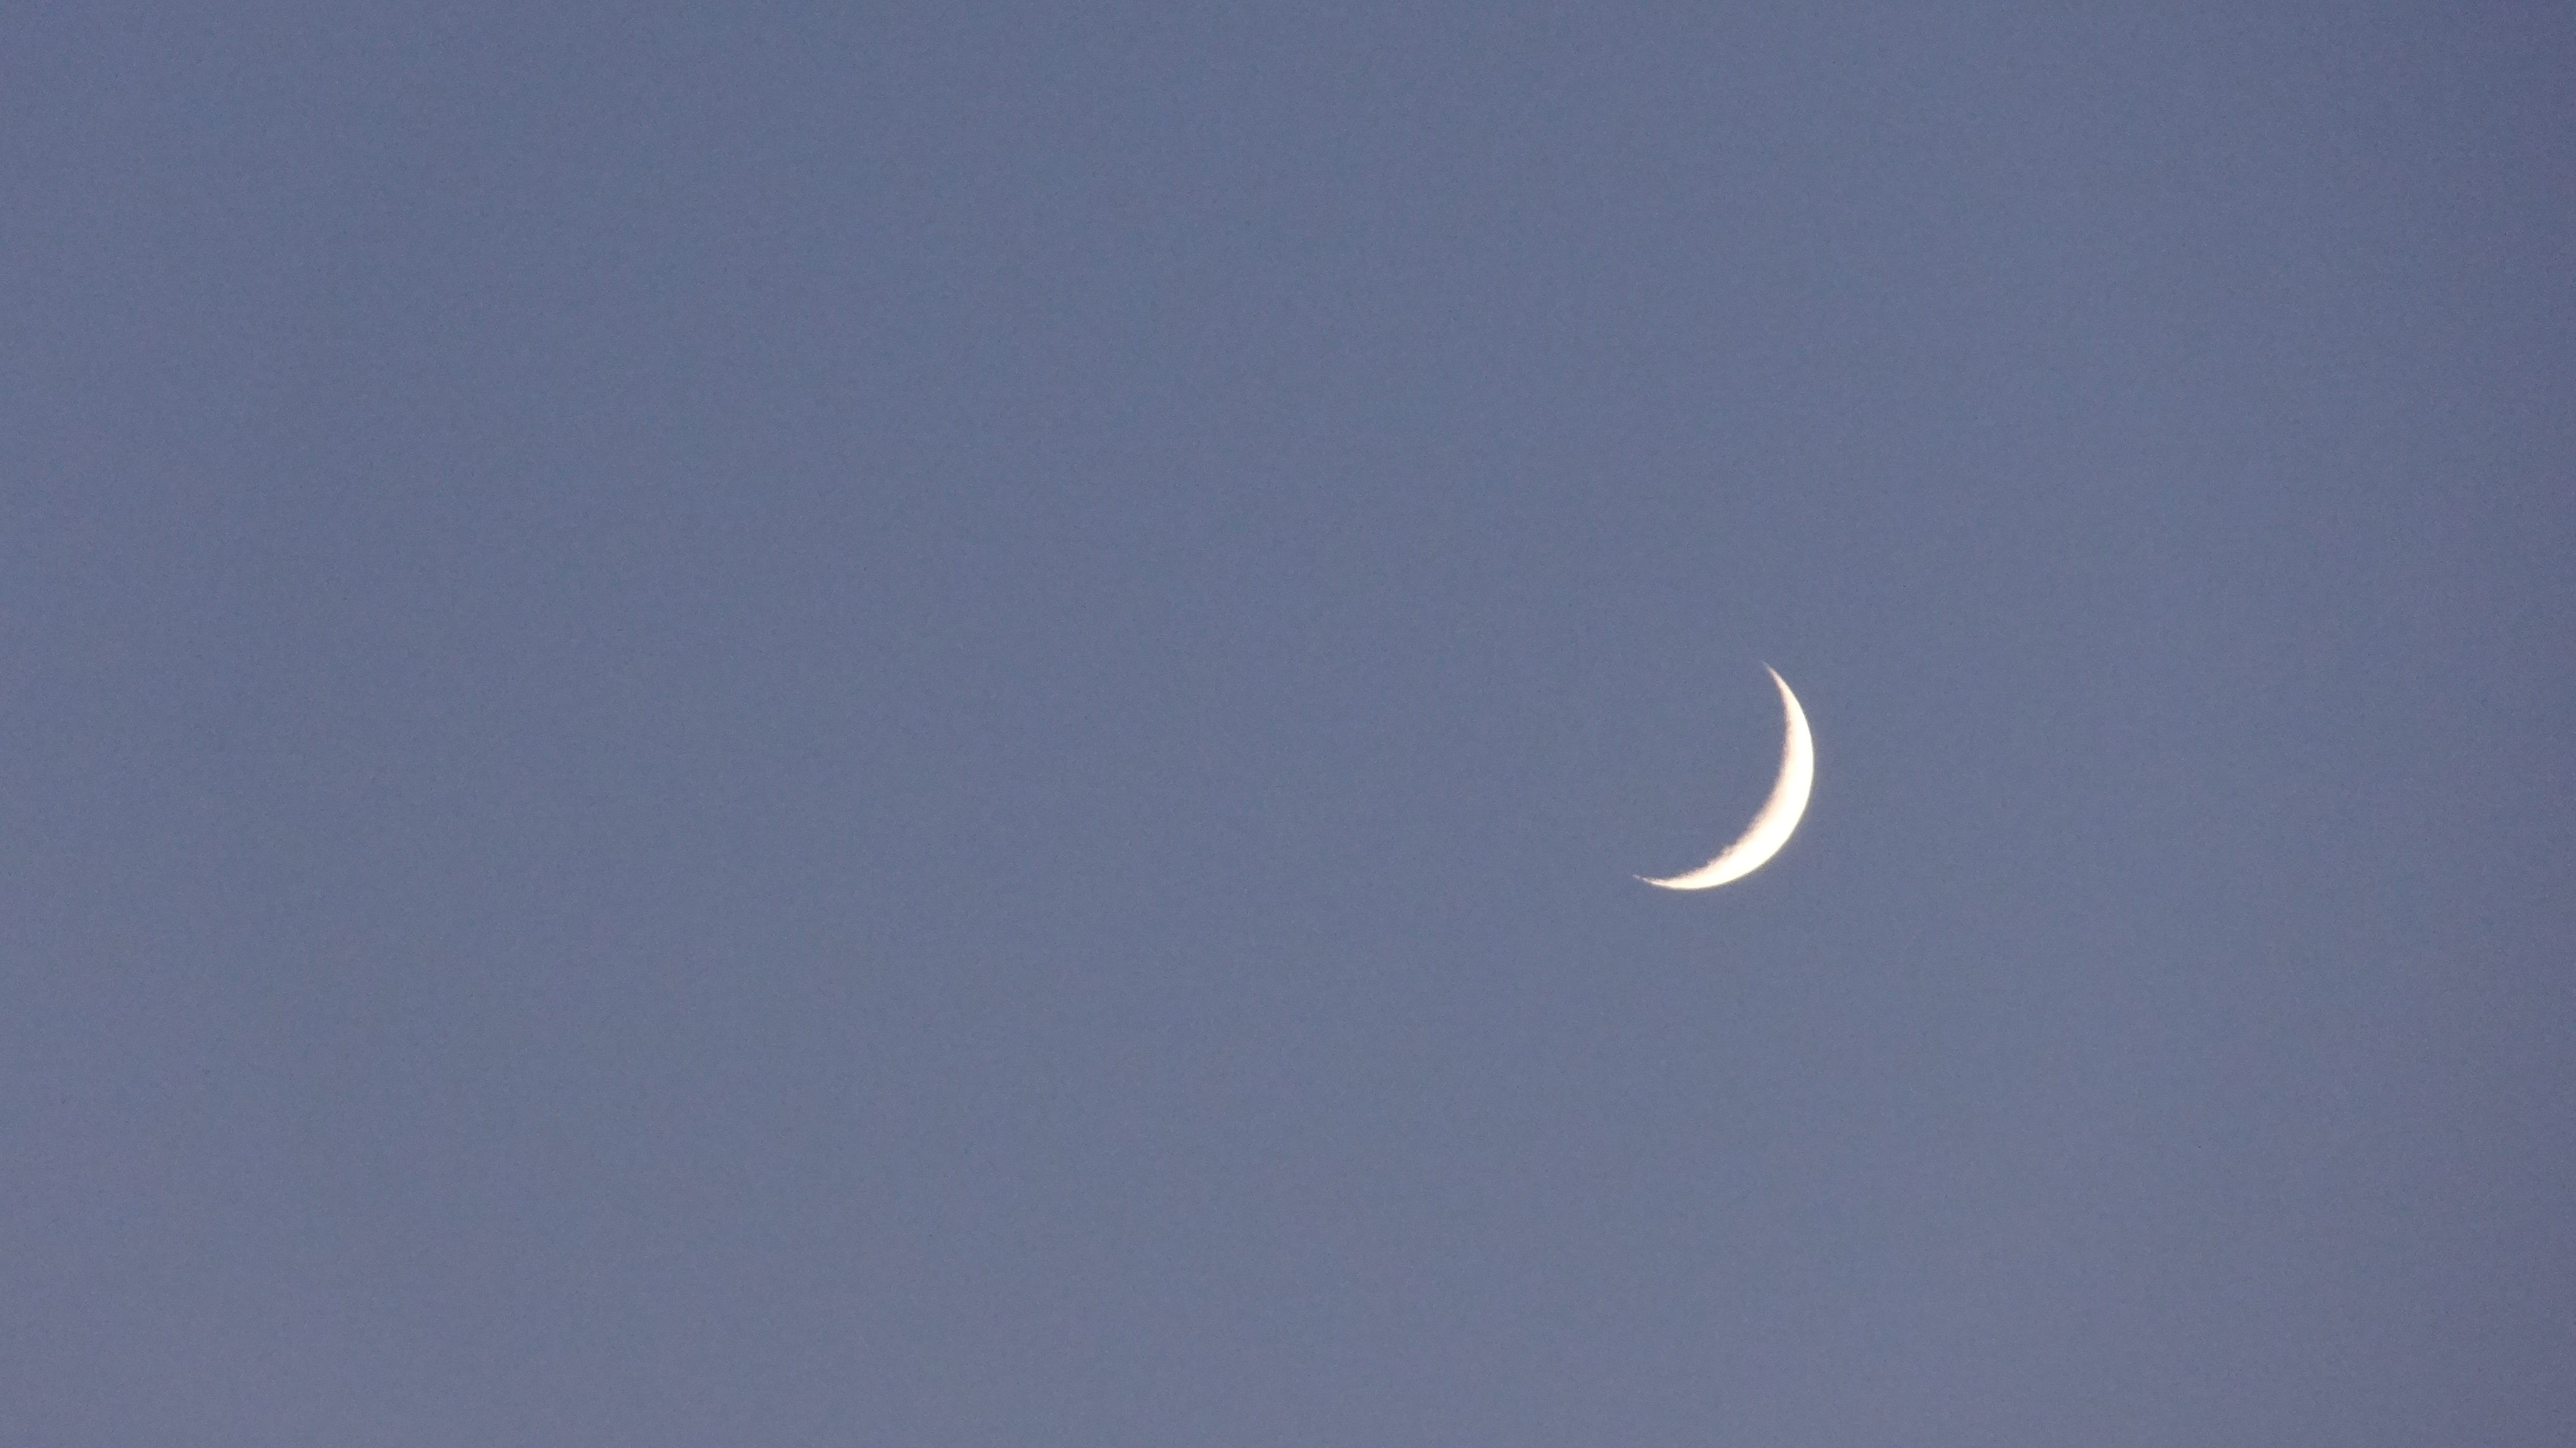
\includegraphics[width=0.5\linewidth]{pictures/DSC00685.JPG}
    \caption{Wieczorne niebo}
    \label{fig:niebo}
\end{figure}

\subsection{Lista numerowana: }
Żeby grupa istniała:
\begin{enumerate}
    \item musi mieć działanie wewnętrzne
    \item działanie musi być łączne
    \item dla każdego elementu grupy musi istnieć element symetryczny
    \item istnieje element neutralny
\end{enumerate}

\subsection{Lista nienumerowana: }
Ciasto na pizze zrobisz z:
\begin{enumerate}
    \item Mąka typ 00
    \item Woda
    \item Drożdże
    \item Sól
    \item Cukier
\end{enumerate}

\subsection{Tekst: }
    \justifying
    \noindent Oto jest przykład krótkiego tekstu z kilkoma formatowaniami.
    Trzeba pamiętać, że pierwszy akapit w nowym rozdziale \textbf{nie ma wcięcia w tekście} - \underline{tak mówią zasady gramatyki języka polskiego.}
    \par
    Kolejny akapit można już zacząć od wcięcia. Latex umożliwia włączenie języka polskiego, więc można cieszyć się naszymi pięknymi literami: \textit{ąćęółżź}.
    Na końcu jeszcze dodam odniesienie do zdjęcia, żeby można było sobie przypomnieć ten piękny widok
    \ref{fig:niebo}.
    Pasowałoby także jeszcze wspomnieć o tej wspaniałej tabeli \ref{fig:tabelka}
\newpage